\chapter{Árboles de decisión. Fundamentos}\label{Chapter6} 
% chktex-file 8
% chktex-file 12
% chktex-file 13
% chktex-file 44

\section{Árboles de decisión}

Esencialmente, este tipo de modelos se basan en la partición recursiva del espacio de características en regiones más pequeñas. En cada paso, se selecciona una característica y un punto de corte, dividiendo el espacio en dos regiones. Este proceso se repite en cada región hasta que se cumple un criterio de parada. La predicción se realiza asignando a cada observación la media o moda de las observaciones de entrenamiento en la región a la que pertenece. \\

Se tratan de modelos altamente interpretables, que no requieren de la normalización de los datos y que pueden manejar tanto variables cualitativas como cuantitativas. Sin embargo, su precisión no es tan alta como la de otros modelos de aprendizaje supervisado. A pesar de ello, mejoran en gran medida cuando se usan en combinación con \textit{bagging} o \textit{boosting}. En este tema, solo veremos CART (\textit{classification and regression tree}). 

\begin{example}
Usamos un conjunto de datos con dos predictores y una variable dependiente cuantitativa. En la figura (\ref{fig:6.1}) se muestra un árbol de decisión ajustado a estos datos. En la primera división, el espacio de predictores se divide en dos regiones, una región donde $X_j < t_k$ y otra donde $X_j \geq t_k$. 
\begin{figure}[h]
\centering
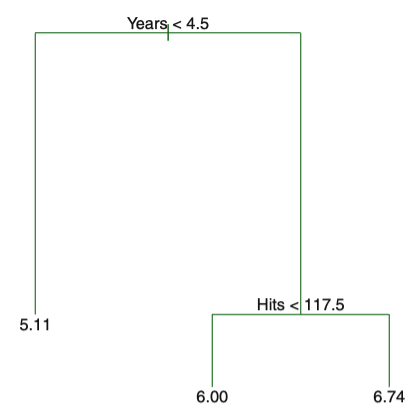
\includegraphics[width=0.5\textwidth]{fotos/31.png}
\caption{Árbol de decisión para un problema de regresión. En un nodo $X_j < t_k$, la rama izquierda representa la región donde se cumple la condición y la rama derecha la región donde no se cumple ($X_j \geq t_k$).}
\label{fig:6.1}
\end{figure}

\begin{figure}[h]
\centering
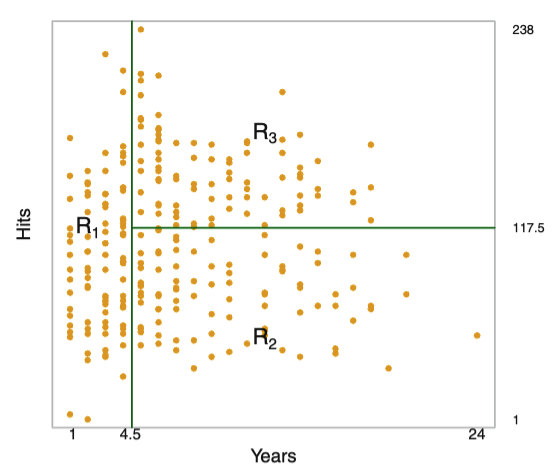
\includegraphics[width=0.5\textwidth]{fotos/32.png}
\caption{La partición de tres regiones del árbol de regresión mostrado en la figura \ref{fig:6.1}.}
\label{fig:6.2}
\end{figure}
Estas tres regiones se pueden escribir como $R_1 = \{X | \text{Years} < 4.5\}$, $R_2 = \{X | \text{Years} \geq 4.5, \text{Hits} < 117.5\}$, y $R_3 = \{X | \text{Years} \geq 4.5, \text{Hits} \geq 117.5\}$. De acuerdo con la analogía del árbol, las regiones $R_1$, $R_2$, y $R_3$ son conocidas como nodos terminales o hojas del árbol. Como en el caso de la figura \ref{fig:6.1}, los árboles de decisión usualmente se dibujan al revés, en el sentido de que las hojas están en la parte inferior del árbol. Los puntos a lo largo del árbol donde el espacio de predictores se divide se conocen como nodos internos. En la figura \ref{fig:6.1}, los dos nodos internos son indicados por el texto \textit{Years} < 4.5 y \textit{Hits} < 117.5. Nos referimos a los segmentos de los árboles que conectan los nodos como ramas. Podríamos interpretar el árbol de regresión mostrado en la figura \ref{fig:6.1} de la siguiente manera: \textit{Years} es el factor más importante para determinar el salario, y los jugadores con menos experiencia ganan salarios más bajos que los jugadores con más experiencia. Dado que un jugador tiene menos experiencia, el número de \textit{hits} que obtuvo en el año anterior parece jugar poco papel en su salario. Pero entre jugadores que han estado en las ligas mayores por cinco o más años, el número de \textit{hits} obtenidos en el año anterior sí afecta el salario, y los jugadores que obtuvieron más \textit{hits} el año pasado tienden a tener salarios más altos. 
\end{example}



\subsection{Predicción mediante estratificación del espacio de características}

Ahora discutimos el proceso de construcción de un árbol de regresión. En términos generales,
hay dos pasos.
\begin{enumerate}
\item Dividimos el espacio de predictores, es decir, el conjunto de posibles valores para $X_1, X_2, \ldots, X_p$, en $J$ regiones distintas y no superpuestas, $R_1, R_2, \ldots, R_J$.
\item Para cada observación que cae en la región $R_j$, hacemos la misma predicción, que es simplemente la media de los valores de respuesta para los datos de entrenamiento en $R_j$.
\end{enumerate}

Veamos ahora como construir las regiones $R_1, \ldots, R_J$. En teoría, las regiones podrían tener cualquier forma. Sin embargo, elegimos dividir el espacio de predictores en rectángulos de alta dimensión, o cajas, para simplicidad y para facilitar la interpretación del modelo predictivo resultante. El objetivo es encontrar cajas $R_1, \ldots, R_J$ que minimicen el RSS, dado por
\begin{equation}
\sum_{j=1}^{J} \sum_{i \in R_j} (y_i - \hat{y}_{R_j})^2 
\end{equation}

donde $\hat{y}_{R_j}$ es la media de respuesta para las observaciones de entrenamiento dentro de la $j$-ésima caja. Desafortunadamente, es computacionalmente inviable considerar cada partición posible del espacio de características en $J$ cajas. \\

Por esta razón, tomamos un enfoque voraz de arriba hacia abajo conocido como división binaria recursiva. El enfoque es de arriba hacia abajo porque comienza en la parte superior del árbol (en ese punto todas las observaciones pertenecen a una sola región) y luego divide sucesivamente el espacio de predictores; cada división se indica mediante dos nuevas ramas más abajo en el árbol. Es voraz porque en cada paso del proceso de construcción del árbol, la mejor división se realiza en ese paso en particular, en lugar de mirar hacia adelante y elegir una división que conducirá a un árbol mejor en algún paso futuro. Para realizar la división binaria recursiva:
\begin{itemize}
\item Primero, seleccionamos el predictor $X_j$ y el punto de corte $s$ tal que dividir el espacio de predictores en las regiones $\{X \mid X_j < s\}$ y $\{X \mid X_j \geq s\}$ conduce a la mayor reducción posible en el RSS en cada región. Es decir, consideramos todos los predictores $X_1, \ldots, X_p$, y todos los posibles valores del punto de corte $s$ para cada uno de los predictores, y luego elegimos el predictor y punto de corte tal que el árbol resultante tenga el RSS más bajo. Con mayor detalle, para cualquier $j$ y $s$, definimos el par de semiplanos
\begin{equation}
R_1(j, s) = \{X \mid X_j < s\} \quad \text{y} \quad R_2(j, s) = \{X \mid X_j \geq s\}
\end{equation}
\noindent y buscamos el valor de $j$ y $s$ que minimice la ecuación
\begin{equation}
\sum_{i: x_i \in R_1(j, s)} (y_i - \hat{y}_{R_1})^2 + \sum_{i: x_i \in R_2(j, s)} (y_i - \hat{y}_{R_2})^2
\end{equation}
donde $\hat{y}_{R_1}$ es la media de respuesta para las observaciones de entrenamiento en $R_1(j, s)$, y $\hat{y}_{R_2}$ es la media de respuesta para las observaciones de entrenamiento en $R_2(j, s)$. Encontrar los valores de $j$ y $s$ que minimicen esta ecuación se puede hacer bastante rápido, especialmente cuando el número de características $p$ no es demasiado grande.
\item Repetimos el proceso, buscando el mejor predictor y mejor punto de corte para dividir los datos aún más de manera que minimicemos el RSS dentro de cada una de las regiones resultantes. Sin embargo, esta vez, en lugar de dividir el todo el espacio de predictores, dividimos una de las dos regiones previamente identificadas. 
\item El proceso continúa hasta que se alcanza un criterio de parada; por ejemplo, podemos continuar hasta que ninguna región contenga más de cinco observaciones (\textit{minimum node size}), hasta llega a cierta profundidad (\textit{maximum depth}).
\item Una vez que las regiones $R_1, \ldots, R_J$ han sido creadas, predecimos la respuesta para una observación de prueba dada usando la media de las observaciones de entrenamiento en la región a la que pertenece dicha observación de prueba. Un ejemplo de cinco regiones de este enfoque se muestra en la figura \ref{fig:6.3}.
\begin{figure}[H]
\centering
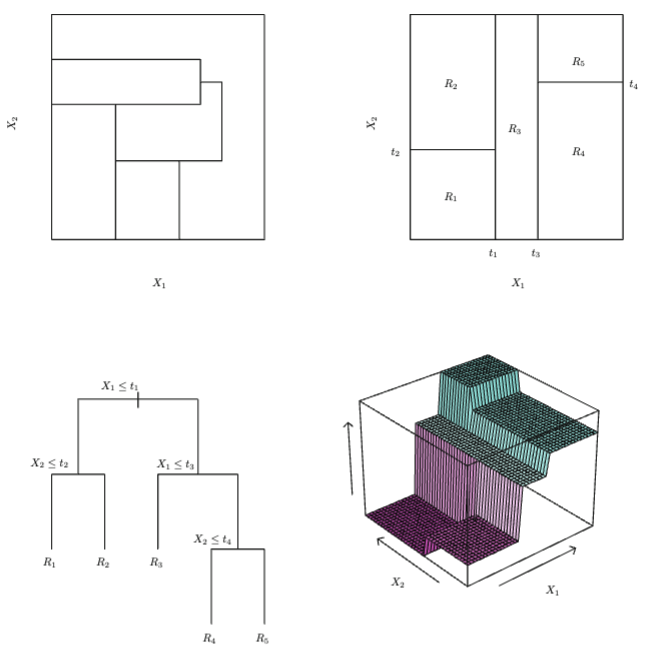
\includegraphics[width=0.7\textwidth]{fotos/33.png}
\caption{Arriba a la izquierda se tiene una particioón de un espacio de características bidimensional que no puede ser nunca resultado de una división binaria recursiva. Arriba a la derecha se tiene un ejemplo de división binaria recursiva. Abajo tenemos el correspondiente árbol y la superficie del mismo.}
\label{fig:6.3}
\end{figure}
\end{itemize}

\subsection{Poda del árbol}

El proceso descrito anteriormente puede producir buenas predicciones en el conjunto
de entrenamiento, pero es probable que sobreajuste los datos, dando un desempeño pobre en el conjunto de prueba. Esto se debe a que el árbol resultante podría ser demasiado complejo. Un árbol más pequeñ con menos divisiones (es decir, menos regiones $R_1, \ldots, R_J$) podría llevar a una menor varianza y mejor interpretación a costa de un poco de sesgo. \\

Una posible alternativa al proceso descrito anteriormente es construir el árbol solo mientras la disminución en el RSS debido a cada división exceda algún umbral (alto). Esta estrategia resultará en árboles más pequeños, pero es demasiado miope ya que una división aparentemente inútil al inicio del árbol podría ser seguida por una división muy buena, es decir, una división que conduce a una gran reducción en el RSS más adelante. Por lo tanto, una mejor estrategia es crecer un árbol muy grande $T_0$, y luego podiarlo para obtener un subárbol. Intuitivamente, nuestro objetivo es seleccionar un subárbol que conduzca a la tasa de error de prueba más baja. Dado un subárbol, podemos estimar su error de prueba usando validación cruzada o el enfoque de conjunto de validación. Sin embargo, estimar el error de validación cruzada para cada subárbol posible sería demasiado cargoso, ya que hay un número extremadamente grande de subárboles posibles. \\

En cambio, necesitamos una forma de seleccionar un pequeño conjunto de subárboles para consideración. La poda de complejidad de costo, también conocida como poda del eslabón más débil, nos da una manera de hacer precisamente esto. En lugar de considerar cada subárbol posible, consideramos una secuencia de árboles indexados por un parámetro de ajuste no negativo $\alpha$. Para cada valor de $\alpha$ corresponde un subárbol $T \subset T_0$ tal que
\begin{equation}
\sum_{m=1}^{|T|} \sum_{i: x_i \in R_m} (y_i - \hat{y}_{R_m})^2 + \alpha |T|
\label{eq:6.4}
\end{equation} 
es lo más pequeño posible. Aquí $|T|$ indica el número de nodos terminales del árbol $T$, $R_m$ es el rectángulo (es decir, el subconjunto del espacio de predictores) correspondiente al $m$-ésimo nodo terminal, y $\hat{y}_{R_m}$ es la respuesta predicha asociada con $R_m$, es decir, la media de las observaciones de entrenamiento en $R_m$. \\

El parámetro de ajuste $\alpha$ controla una compensación entre la complejidad del subárbol y su ajuste a los datos de entrenamiento. Cuando $\alpha = 0$, entonces el subárbol $T$ simplemente igualará a $T_0$, porque entonces la ecuación solo mide el error de entrenamiento. Sin embargo, a medida que $\alpha$ aumenta, hay un costo por tener un árbol con muchos nodos terminales, por lo que la cantidad (\ref{eq:6.4}) tenderá a ser minimizada para un subárbol más pequeño. La ecuación (\ref{eq:6.4}) es similar a Lasso, donde buscamos controlar la complejidad de un modelo lineal. \\

Resulta que al aumentar $\alpha$ desde cero en (\ref{eq:6.4}), las ramas se podan del árbol de manera anidada y predecible, por lo que obtener toda la secuencia de subárboles en función de $\alpha$ es fácil. Podemos seleccionar un valor de
$\alpha$ usando un conjunto de validación o usando validación cruzada. Luego, volvemos al conjunto de datos completo y obtenemos el subárbol correspondiente a $\alpha$. Hagamos un resumen de este proceso:
\begin{enumerate}
\item Usar divisón binaria recursiva para hacer crecer un árbol grande para los datos de entrenamiento y parar cuando cada nodo terminal tenga menos de un número mínimo de observaciones.
\item Aplicar la poda de complejidad de costo para obtener una secuencia de subárboles como una función de $\alpha$.
\item Usar validación cruzada para seleccionar $\alpha$. Esto es, dividir los datos de entrenamiento en $K$ grupos. Para cada $k = 1, 2, \ldots, K$:
\begin{enumerate}
\item Repetir los pasos 1 y 2 en todos los grupos menos el k-ésimo.
\item Evaluar el MSE de los datos del grupo k-ésimo, como función de $\alpha$. 
\end{enumerate}
Promediar los resultados para cada valor de $\alpha$ y coger el $\alpha$ que minimice el error medio.
\item Devolver el subárbol del paso 2 que corresponda al valor escogido de $\alpha$.
\end{enumerate}

Las figuras \ref{fig:6.4} y \ref{fig:6.5} muestran los resultados de ajustar y podar un árbol de regresión en ciertos datos, usando nueve de las características.

\begin{figure}[h]
\centering
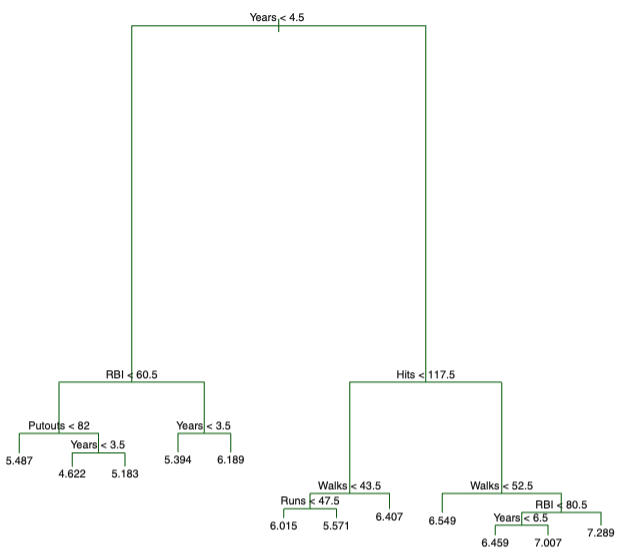
\includegraphics[width=0.5\textwidth]{fotos/34.png}
\caption{Árbol de regresión sin podar.}
\label{fig:6.4}
\end{figure}

\begin{figure}[h]
\centering
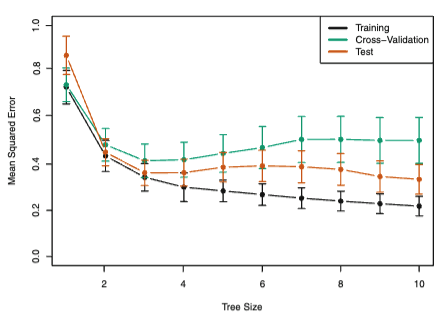
\includegraphics[width=0.5\textwidth]{fotos/35.png}
\caption{El mínimo error de de validación cruzada (hecha con 6 grupos) se da para un tamaño de árbol de tres. El árbol podado que contiene tres nodos terminales se muestra en la figura \ref{fig:6.1}.}
\label{fig:6.5}
\end{figure}


\subsection{Árboles de Clasificación}

Un árbol de clasificación es muy similar a un árbol de regresión, excepto que se usa para predecir una respuesta cualitativa en lugar de una cuantitativa. En contraste a los de regresión, para un árbol de clasificación, predecimos que cada observación pertenece a la clase más ocurrida de las observaciones de entrenamiento en la región a la que pertenece. \\

Al interpretar los resultados de un árbol de clasificación, a menudo nos interesa no solo la predicción de la clase correspondiente a una región particular del nodo terminal, sino también las proporciones de clase entre las observaciones de entrenamiento que caen en esa región. \\

La tarea de construir un árbol de clasificación es bastante similar a la tarea de construir un árbol de regresión. Al igual que en el entorno de regresión, usamos división binaria recursiva para construir un árbol de clasificación. Sin embargo, en el entorno de clasificación, el RSS no puede ser usado como criterio para hacer las divisiones binarias. Una alternativa natural al RSS es la tasa de error de clasificación. Dado que planeamos asignar una observación en una región dada a la clase más comúnmente ocurrida de las observaciones de entrenamiento en esa región, la tasa de error de clasificación es simplemente la fracción de las observaciones de entrenamiento en esa región que no pertenecen a la clase más común.
\begin{equation}
E = 1 - \max_k (\hat{p}_{mk})
\end{equation}

Aquí, $\hat{p}_{mk}$ representa la proporción de observaciones de entrenamiento en la $m$-ésima región que pertenecen a la $k$-ésima clase. Sin embargo, resulta que el error de clasificación no es suficientemente sensible para el crecimiento del árbol, y en la práctica dos otras medidas son preferibles: 

\begin{itemize}
\item El índice de Gini se define por
\begin{equation}
G = \sum_{k=1}^{K} \hat{p}_{mk}(1 - \hat{p}_{mk})
\end{equation}
una medida de la varianza total a través de las $K$ clases. No es difícil ver que el índice de Gini toma un valor pequeño si todas las $\hat{p}_{mk}$ están cerca de cero o uno. Por esta razón, el índice de Gini se conoce como una medida de pureza del nodo; un valor pequeño indica que un nodo contiene predominantemente observaciones de una sola clase.
\item Una alternativa al índice de Gini es la entropía cruzada, dada por 
\begin{equation}
D = -\sum_{k=1}^{K} \hat{p}_{mk} \log \hat{p}_{mk}
\end{equation}
ya que $0 \leq \hat{p}_{mk} \leq 1$, se sigue que $0 \leq -\hat{p}_{mk} \log \hat{p}_{mk}$. Se puede demostrar que
la entropía cruzada tomará un valor cercano a cero si las $\hat{p}_{mk}$ están todas cerca de cero o cerca de uno. Por lo tanto, al igual que el índice de Gini, la entropía cruzada tomará un valor pequeño si el $m$-ésimo nodo está puro. De hecho, resulta que el índice de Gini y la entropía cruzada son bastante similares numéricamente.
\end{itemize}

\begin{figure}[h]
\centering
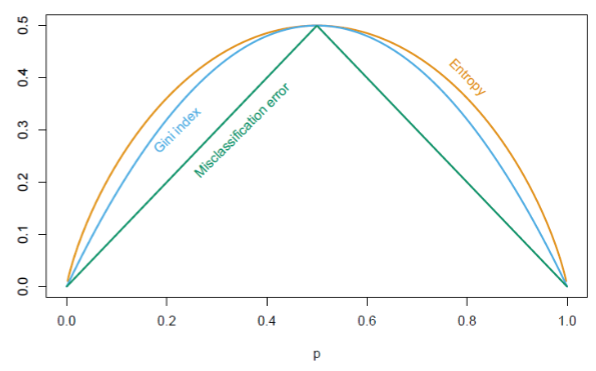
\includegraphics[width=0.5\textwidth]{fotos/38.png}
\caption{Medidas usadas como criterio de división en árboles de clasificación en función de la probabilidad. Medidas de impureza de nodos para clasificación binaria (la entropía cruzada se ha escalado).}
\label{fig:6.66}
\end{figure}

Al construir un árbol de clasificación, típicamente se usa el índice de Gini o la entropía cruzada para evaluar la calidad de una división particular, ya que estos dos enfoques son más sensibles a la pureza del nodo que la tasa de error de clasificación (figura \ref{fig:6.66}). Cualquiera de estos tres enfoques podría ser usado al podar el árbol, pero la tasa de error de clasificación es preferible si el objetivo es la precisión predictiva del árbol podado final. \\

\begin{figure}[h]
\centering
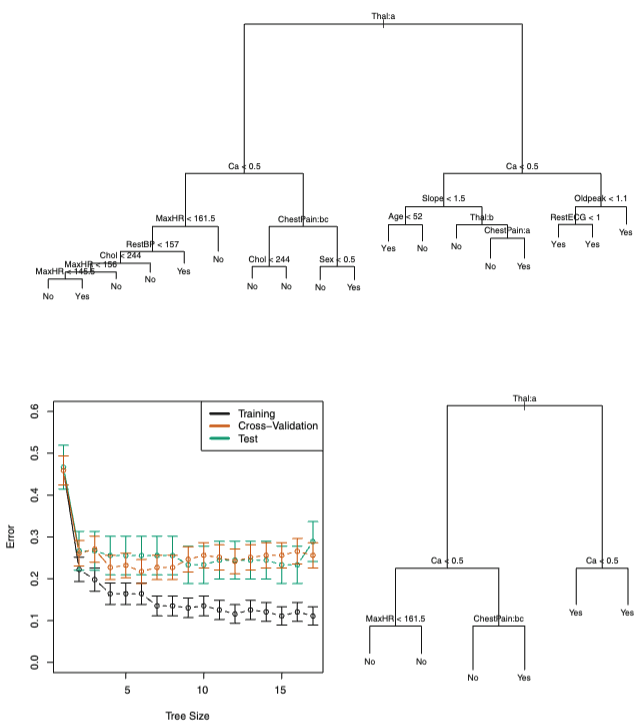
\includegraphics[width=0.5\textwidth]{fotos/36.png}
\caption{Estos datos contienen un resultado binario HD para 303 pacientes que se presentaron con dolor en el pecho. Un valor de resultado de Sí indica la presencia de enfermedad cardíaca basada en una prueba angiográfica, mientras que No significa ausencia de enfermedad cardíaca. Hay 13 predictores incluyendo \textit{Age}, \textit{Sex}, \textit{Chol} (una medida de colesterol), y otras medidas de función cardíaca y pulmonar. La validación cruzada resulta en un árbol con seis nodos terminales. Algunos predictores son cualitativos: las divisiones sobre estas variables equivalen a asignar algunos de los valores cualitativos a una rama y asignar los restantes a la otra rama. El texto \textit{Thal:a} indica que la rama izquierda que sale de ese nodo consiste en observaciones con el primer valor de la variable \textit{Thal} (normal), y el nodo derecho
consiste en las observaciones restantes (defectos fijos o reversibles). El texto \textit{ChestPain:bc} dos divisiones hacia abajo en el árbol a la izquierda indica que la rama izquierda que sale de ese nodo consiste en observaciones con el segundo y tercer valor de la variable \textit{ChestPain}, donde los posibles valores son angina típica, angina atípica, dolor no anginoso, y asintomático.}
\label{fig:6.7}
\end{figure}

La figura \ref{fig:6.7} muestra un ejemplo en un conjunto de datos. \\

En nuestra discusión hasta ahora, hemos asumido que las variables de predictores toman valores continuos. Sin embargo, se pueden construir árboles de decisión incluso en presencia de variables de predictores cualitativas. De hecho, son el único método de aprendizaje estadístico capaz de manejar este tipo de variable de forma natural. \\

La figura \ref{fig:6.7} muestra como algunas de las divisiones generan dos nodos terminales que tienen el mismo valor predicho. Por ejemplo, consideremos la división \textit{RestECG} $<$ 1 cerca de la parte inferior derecha del árbol sin podar. Independientemente del valor de \textit{RestECG}, se predice un valor de Sí para esas observaciones. ¿Por qué, entonces, se realiza la división? La división se realiza porque conduce a una mayor pureza del nodo. Es decir, las 9 observaciones correspondientes a la hoja derecha tienen un valor de respuesta de Sí, mientras que 7/11 de las correspondientes a la hoja izquierda tienen un valor de respuesta de Sí. ¿Por qué es importante la pureza del nodo? Supongamos que tenemos una observación de prueba que pertenece a la región dada por esa hoja derecha. Entonces podemos estar bastante seguros de que su valor de respuesta es Sí. En contraste, si una observación de prueba pertenece a la región dada por la hoja izquierda, entonces su valor de respuesta es probablemente Sí, pero somos mucho menos ciertos. Aunque la división \textit{RestECG} $<$ 1 no reduce el error de clasificación, mejora el índice de Gini y la entropía cruzada, que son más sensibles a la pureza del nodo.

\subsection{Predictores categóricos}

Sean $q$ valores, o niveles, de una variable predictora cualitativa. Podemos crear $2^q - 1$ divisiones binarias posibles de los $q$ niveles. En un problema de dos clases (binario), se ordenan las clases del predictor según la proporción que tiene como salida 1. Posteriormente, se divide como un predictor ordenado y se toma la división óptima en términos del índice de Ginny o la entropía cruzada. \\

Esto también aplica para regresión, haciendo uso del RSS. Sin embargo, aquí se ordenan las categorías de forma creciente según la media de la salida. \\

Para salidas multicategóricas, esta simplificación no es posible. En general, hay que evitar varibales con un gran $q$, ya que generan sobreajuste.

\begin{example}
Sea una variable con cuatro posibles valores ($q = 4$) $X_1 = (A, B, C, D)$, para particionar podemos hacerlo del 7 formas distintas: 
\begin{equation}
\{(A, BCD), (B, ACD), (C, ABD), (D, ABC), (AB, CD), (AC, BD), (AD, BC)\}
\end{equation}
Podemos reducir el numero de particiones a calcular: sea $X_1 \in (A, B, C, D)$. Supongamos que de los ejemplos de $X_1 = A$, $p_+ = 0.2$ y $p_- = 0.8$. Para $X_1 = B$, $p_+ = 0.3$ y $p_- = 0.7$. Para $X_1 = C$, $p_+ = 0.4$ y $p_- = 0.6$. Para $X_1 = D$, $p_+ = 0.1$ y $p_- = 0.9$. 

Ahora, ordenamos en orden creciente de la clase positiva. El valor más bajo es D con $0.1$, el siguiente A con $0.2$, luego B con $0.3$ y finalmente C con $0.4$. Analizando umbrales ahora (que serían tres), garantizamos solución optima en cuanto a Ginny y entropia cruzada. Esta simplificación solo es válida para clasificación binaria, independientemente de $q$. Para clasificación multicategórica hay que probar todas las posibles particiones sin hacer este truco de reducir.
\end{example}

\subsection{Árboles vs Modelos lineales}

Los árboles de regresión y clasificación son muy diferentes respecto a los enfoques más clásicos para regresión y clasificación. En particular, la regresión lineal asume un modelo de la forma
\begin{equation}
f(X) = \beta_0 + \sum_{j=1}^{p} X_j \beta_j
\end{equation}

\noindent mientras que los árboles de regresión asumen un modelo de la forma
\begin{equation}
f(X) = \sum_{m=1}^{M} c_m \cdot 1_{(X \in R_m)}
\end{equation}

donde $R_1, \ldots, R_M$ representan una partición del espacio de características. Si la relación entre los predictores y la respuesta está bien aproximada por un modelo lineal, entonces un enfoque como la regresión lineal probablemente funcionará bien, y superará a un método como un árbol de regresió que no explota esta estructura lineal. Si, en cambio, existe una relación altamente no lineal y compleja entre los predictores y la respuesta, entonces los árboles de decisión pueden superar a los enfoques clásicos. Un ejemplo ilustrativo se muestra en la figura \ref{fig:6.88}. 

\begin{figure}[h]
\centering
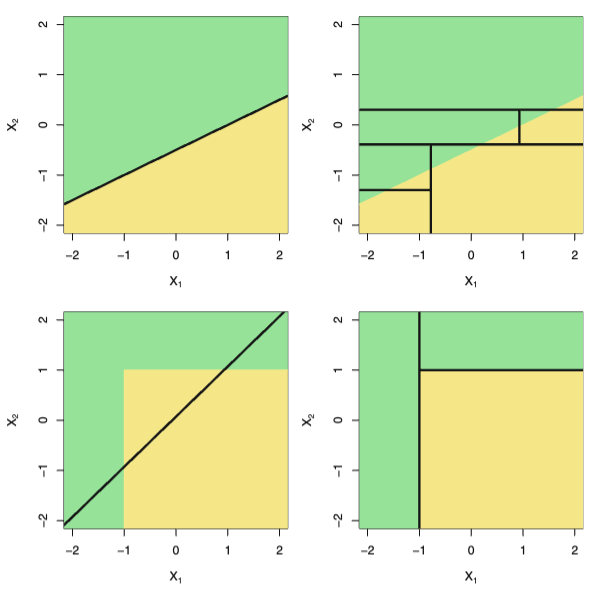
\includegraphics[width=0.5\textwidth]{fotos/37.png}
\caption{Ejemplos donde regresión lineal es preferible sobre árboles de decisión y viceversa.}
\label{fig:6.88}
\end{figure}

\subsection{Ventajas y desventajas de los árboles}

El tamaño del árbol es el hiperparametro que controlará el subaprendizaje o subaprendizaje del algoritmo. Un árbol pequeño estará subaprendido, y uno grande sobreaprendido. \\

Los árboles de decisión para regresión y clasificación tienen una serie de ventajas sobre los enfoques más clásicos vistos:
\begin{itemize}
    \item Los árboles son muy fáciles de explicar a las personas.
    \item Algunas personas creen que los árboles de decisión reflejan más de cerca el proceso de toma de decisiones humano que los enfoques de regresión y clasificación.
    \item Los árboles pueden ser mostrados gráficamente y son fácilmente interpretados incluso por un no experto (especialmente si son pequeños).
    \item Los árboles pueden manejar fácilmente predictores cualitativos sin la necesidad de crear variables \textit{dummy}.
    \item Desafortunadamente, los árboles generalmente no tienen el mismo nivel de precisión predictiva que algunos de los otros enfoques de regresión y clasificación.
\end{itemize}

Sin embargo, al agregar muchos árboles de decisión, usando métodos como \textit{bagging}, bosques aleatorios y \textit{boosting}, el desempeño predictivo de los árboles puede ser sustancialmente mejorado. 

\section{Ejercicio}

\begin{example}
\textbf{Sea el siguiente conjunto de datos de clasificación con 6 observaciones, 2 variables de entrada y una variable de salida:}
\begin{table}[H]
\centering
\begin{tabular}{cccc}
\hline \hline
Observación & $X_1$ & $X_2$ & $Y$ \\ \hline \hline
1 & 4 & 3 & 1 \\
2 & -3 & -1 & 0 \\
3 & 3 & -2 & 0 \\
4 & 1 & 4 & 1 \\
5 & -2 & 3 & 0 \\
6 & -3 & 5 & 0 \\ \hline
\end{tabular}
\end{table}
\textbf{Construye el árbol de clasificación (sin podar) mediante CART y utilizando como criterio la entropía. La condición de parada debe ser que los nodos hoja sean puros (todos los ejemplos son de la misma clase). En cada nodo del árbol se debe indicar:}
\begin{enumerate}
\item \textbf{La variable y su valor umbral.}
\item \textbf{La entropía correspondiente.}
\item \textbf{En los nodos hoja, la clase del nodo y los ejemplos que pertenecen al mismo.}
\end{enumerate}
\textbf{No es necesario estandarizar las variables.} \\

Básicamente calcular la entropía para todos los umbrales y para todas las características y ver la menor. La primera división se ve que debe hacerse en $X_1 = -0.5$, ya que deja un nodo puro de 3 ejemplos. Su entropía sería:
\begin{equation}
S = \frac{3}{6}\left(-\cancel{0\log 0}^{\; 0} - 1\cancel{\log 1}^{\; 0}\right) + \frac{3}{6}\left(-\frac{1}{3}\log \frac{1}{3} - \frac{2}{3}\log \frac{2}{3}\right) \approx 0.3182570841
\end{equation}

donde $\log$ es el logarítmo natural o neperiano (sí, terrible eso de hacer $0\cdot \log 0 = 0$). El nodo de la derecha lo podemos dividir más. Hay una división que deja dos nodos puros ($X_2 = 0.5$), por lo que esa es la mejor opción ya que tiene entropía nula ($S = 0$). Así, el árbol queda:
\begin{figure}[H]
\centering
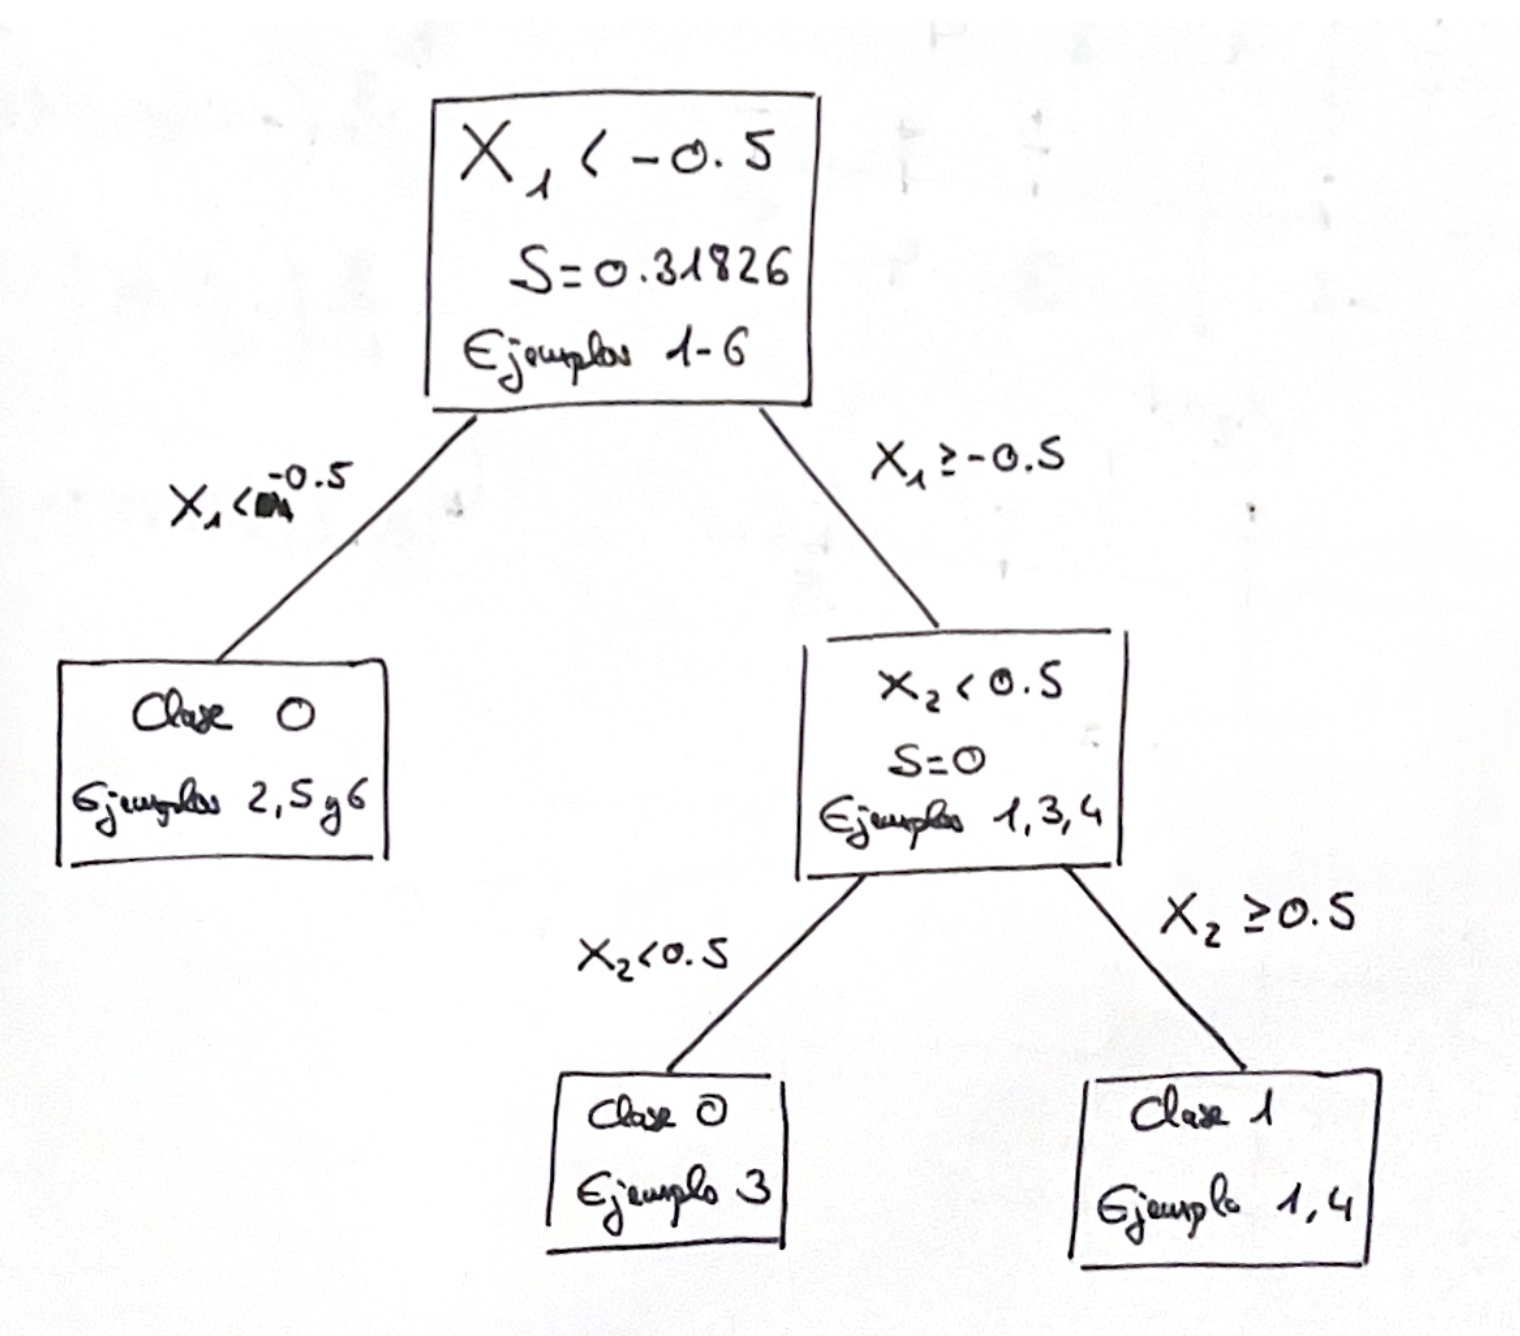
\includegraphics[width=0.6\textwidth]{fotos/39.png}
\end{figure}
\end{example}